\section{Produkteinsatz}

In diesem Abschnitt wird der geplante Einsatz des Systems beschrieben, wobei
insbesondere auf die Systemumgebung, in der das Produkt eingesetzt werden soll,
und die Zuordnung der Software zu dieser eingegangen wird. 
Abbildung \ref{ProdukteinsatzKomp}
zeigt ein Verteilungsdiagramm des Gesamtsystems, dessen Komponenten im Folgenden
erläutert werden.

Das Gesamtsystem besteht im Wesentlichen aus einem \emph{Server}, der mit mindestens einer
\emph{Robot Unit} verbunden ist. Zwischen \emph{Server} und \emph{Robot Units} kann über
einen auf beiden Seiten verfügbaren \emph{Wlan\-Adapter} über ein
Funknetzwerk kommuniziert werden.

Auf dem \emph{Server} und den \emph{Robot Units} läuft ein \emph{Java Runtime Environment},
das dem Ausführen der entsprechenden Software dient.

\emph{RobotUnit.jar} dient der Kapselung aller verfügbaren Funktionen. Es bietet Zugriff
auf \emph{RobotSoftware} und \emph{Robot}.

\emph{Server.jar} agiert analog zu \emph{Robot.jar} und bietet Zugriff auf alle grundlegenden 
Funktionalitäten von \emph{ServerSoftware}, \emph{Hospital} und \emph{TaxiApp}.

Zusätzlich benötigte Funktionalitäten werden aus dem \emph{Common}-Paket importiert und sind
sowohl bei den \emph{Robot Units} als auch dem \emph{Server} verfügbar.

\begin{figure}[H]
	\centering
	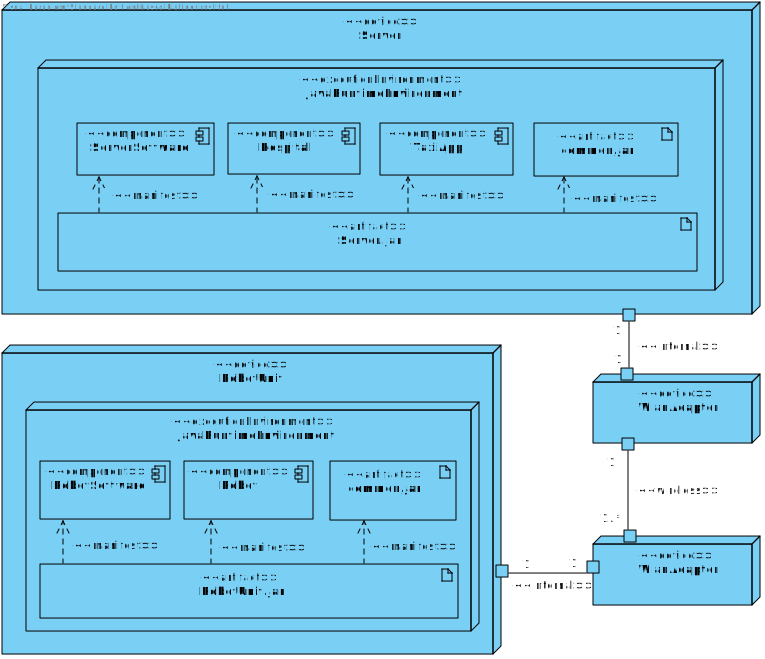
\includegraphics[width=1\textwidth]{img/2-Entwurf-9-Produkteinsatz}
	\caption{Verteilungsdiagramm des Gesamtsystems}
	\label{ProdukteinsatzKomp}
\end{figure}
